\documentclass[showpacs,aps,floatfix,prb,reprint,superscriptaddress]{revtex4-1} 
%\documentclass[showpacs,floatfix,aps,prb,preprint,superscriptaddress]{revtex4-1}
%\documentclass[reprint,aps,groupedaddress]{revtex4-1}
\usepackage{xfrac}
\usepackage{amssymb}
\usepackage{braket}
\usepackage{graphicx}
%\usepackage{floatfix}
\usepackage{verbatim}
\usepackage{etoolbox}
\usepackage{amsfonts} %maths
\usepackage{amsmath} %maths
%\usepackage[fleqn]{amsmath} %maths
\usepackage[utf8]{inputenc} %useful to type directly diacritic characters
\usepackage{mathtools}
\usepackage{soul,xcolor,colortbl}
\usepackage{lipsum}
\usepackage{hyperref} \hypersetup{colorlinks=true,citecolor=blue,linkcolor=blue,urlcolor=blue} % HYPERLINKS
%\usepackage{widetext} %ELSEVIER

 \usepackage{ulem}
\usepackage{bm} %revtex4.1 for bold symbols
\usepackage{array}
\usepackage{color} 


\begin{document}
\title{\Large Ideal Strength and Intrinsic Ductility in Metals and Alloys From Second and Third Order Elastic Constants}
%\author{Maarten de Jong, Mark Asta}
%\affiliation{Department of Materials Science and Engineering, University of California, Berkeley, CA   94720, USA}


\date{\today}

\begin{abstract}
Under tensile loading the ideal strength of a solid is governed by mechanical instabilities corresponding to failure in tension or shear, indicative of intrinsic brittle or ductile behavior, respectively.  First principles-calculations for hexagonal close packed (hcp) metals under tensile loading along the $c$ axis reveal that Be, Mg, Ru, Os and Zn fail in tension, while Sc, Y, Ti, Zr, Hf, Tc and Re fail in shear. An analytical model is developed that predicts this behavior in terms of the second and third order elastic constants. For the transition metals, filling of the $d$-bands is shown to correlate with the type of instability realized, thus providing unique insights into the effect of alloying on the intrinsic mechanical behavior of hcp metals.
\end{abstract}

\maketitle

\section{Introduction}
Intro goes here
%For a given loading condition, the ideal strength of a crystalline solid forms an upper bound on the mechanical stress that the material can sustain prior to reaching a mechanical instability. The nature of the instability reached at this stress level can provide insights into the intrinsic failure mechanisms for a material.  For example, under tensile loading crack initiation requires that the local normal stress perpendicular to the cleavage plane is equal to or larger than the ideal tensile strength \cite{li2007ideal,clatterbuck2003ideal,kelly1986strong,wang2013estimate}.  However, when a material yields under tensile loading, it is possible for it to fail through a shear instability \cite{PhysRevLett.91.135501,PhysRevLett.112.115503,macmillan1983ideal,roundy2001ideal,wang2009elastic}. The tensile versus shear nature of the mechanical instability realized under tensile loading is of considerable interest as an indicator of whether a material will behave in an intrinsically brittle or ductile manner. For cubic metals, first-principles calculations of ideal strength under tensile loading have revealed shear instabilities for the ductile metals V and Nb, whereas more brittle materials such as W and Mo have been shown to fail in tension \cite{PhysRevLett.112.115503}. Similar studies in alloys \cite{PhysRevLett.82.2713,PhysRevB.87.214203,vsob1997theoretical,PhysRevB.58.6006} have been undertaken recently, yielding insights into compositional effects. For example, it has been shown that BCC-based Mo-alloys can be made intrinsically more ductile by tuning the $d$ band filling through alloying \cite{PhysRevLett.112.115503}.
%
%In this work we consider the deformation behavior of the HCP metals, a class of materials that find use in diverse technological applications, spanning biomedical to automotive and aerospace. These materials can possess attractive properties such as high strength-to-weight ratios, high stiffness and/or high melting temperatures. However applications of these materials is often limited by low ductility, associated with the limited number of active slip systems in the HCP structure. Substantial efforts have been devoted to optimizing the ductility of HCP metals and alloys, for example by alloying and through the control of microstructure. Despite this significant body of work, the fundamental ideal strengths of HCP-metals have been reported for only a few systems \cite{fu2012first}, and no attempts at using the results of such studies to derive insights into the intrinsic ductility of these materials, and how they may be altered through alloying, have been made to the best of our knowledge.
%
%For the HCP metals Be, Mg, Sc, Y, Ti, Zr, Hf, Tc, Re, Ru, Os and Zn, we compute the ideal strength and associated mechanical instabilities under tensile loading along the crystallographic $c$ axis, i.e., perpendicular to the basal plane.  This is a particularly important loading condition for the consideration of the intrinsic ductility of HCP metals, as the basal plane is a typical cleavage plane in these materials \cite{yoo1981slip}, and slip of the dominant $a$-type dislocations does not provide a mechanism for plastic elongation along the $c$ direction. Based on the ideal deformation behavior, each of the HCP metals is characterized as intrinsically brittle or ductile, i.e., as  possessing elastic instabilities that are either tensile or shear in nature, respectively. We further study map out domains of $d$-band filling for HCP transition metals where ductile vs brittle behavior can be expected.  Finally, we provide an analytical formalism which enables the ideal strength and the nature of the intrinsic instability under tensile loading along the $c$ axis to be derived solely from a knowledge of the second and third-order elastic elastic constants.  The analytical model is shown to yield predictions in reasonable agreement with explicit density-functional-theory (DFT) calculations across all of HCP metals considered in this work, with reduced computational cost.

\section{Methodology}
\subsection{Derivation of third-order elastic constants for different crystal systems}
In this subsection, consider materials under an applied strain $\xi$, causing a Poisson contraction $\eta$.

\subsubsection{Cubic under uniaxial tension}
State results for cubic symmetry $C'$ for tension along $c$.

\subsubsection{Hexagonal under uniaxial tension}
Consider a hexagonal material under a uniaxial tension along the $c$-axis, thus allowing for Poisson contraction in the basal plane. The expressions for the effective SOEC's are then as given in Eqs. \ref{eqn:Cprime_hexagonal}. Note that for this particular deformation mode, the hexagonal symmetry of the material remains intact and hence, the relation $C_{66} = \frac{1}{2} \left(C_{11} - C_{12}\right)$ holds true along the strain path. 

 \begin{widetext}
\begin{subequations}
\label{eqn:Cprime_hexagonal} 
\begin{align}
        C_{11}' &=C_{11} + \eta \left(3C_{11} + C_{12} + 2C_{222} - 3C_{661} - C_{662}\right) + \xi \left(-C_{11} + C_{23} + C_{223}\right),\\
        C_{12}' &=C_{12} + \eta \left(-C_{11} + C_{12} + 2C_{222} -5C_{661} - 3C_{662}\right) + \xi \left(-C_{12} + C_{223} - C_{23} - 2C_{663}\right),\\
				C_{23}' &=C_{23} + \eta \left(-C_{11}-C_{12}+2C_{223}-2C_{663} \right) + \xi \left(C_{332}\right),\\
				C_{33}' &=C_{33} + \eta \left(2C_{23}-2C_{33}+2C_{332} \right) + \xi \left(4C_{33}+C_{333}\right),\\
				C_{44}' &=C_{44} + \eta \left(\frac{1}{2} C_{11} + \frac{1}{2} C_{12} + C_{23} + C_{551} + C_{552} \right) + \xi \left(\frac{1}{2} C_{23} + \frac{1}{2} C_{33} + C_{44} + C_{553}\right),\\
				C_{66}' &=\frac{1}{2} \left(C_{11}'-C_{12}'\right)
\end{align}
\end{subequations}
\end{widetext} 










\subsubsection{Do we want to include other symmetries?}

\subsection{Calculation of second and third-order elastic constants}

\subsubsection{Cubic symmetry}


\subsubsection{Hexagonal symmetry}

Into SM.
\onecolumngrid

%\begin{equation}
%\label{eqn:s1} 
%t_{1} \left(\eta_{1}\right) = \rho_{0} \frac{\partial E}{\partial \eta_{1}}\Bigr|_{\eta_2=\eta_3=\eta_4=\eta_5=\eta_6=0} = \frac{C_{111}\eta_{1}^2}{2} + C_{11}\eta_{1}
%\end{equation}
%
%\begin{equation}
%\label{eqn:s2} 
%t_{2} \left(\eta_{2}\right) = \rho_{0} \frac{\partial E}{\partial \eta_{2}}\Bigr|_{\eta_1=\eta_3=\eta_4=\eta_5=\eta_6=0} = \frac{C_{222}\eta_{2}^2}{2} + C_{11}\eta_{2}
%\end{equation}
%
%
%\begin{equation}
%\label{eqn:s3} 
%t_{3} \left(\eta_{3}\right) = \rho_{0} \frac{\partial E}{\partial \eta_{3}}\Bigr|_{\eta_1=\eta_2=\eta_4=\eta_5=\eta_6=0} = \frac{C_{333}\eta_{3}^2}{2} + C_{33}\eta_{3}
%\end{equation}
%
%
%\begin{equation}
%\label{eqn:s4} 
%t_{3} \left(\eta_{1}\right) = \rho_{0} \frac{\partial E}{\partial \eta_{3}}\Bigr|_{\eta_2=\eta_3=\eta_4=\eta_5=\eta_6=0} = \frac{C_{113}\eta_{1}^2}{2} + C_{13}\eta_{1}
%\end{equation}
%
%
%\begin{equation}
%\label{eqn:s5} 
%t_{1} \left(\eta_{3}\right) = \rho_{0} \frac{\partial E}{\partial \eta_{1}}\Bigr|_{\eta_1=\eta_2=\eta_4=\eta_5=\eta_6=0} = \frac{C_{133}\eta_{3}^2}{2} + C_{13}\eta_{3}
%\end{equation}
%
%\begin{equation}
%\label{eqn:s6} 
%t_{2} \left(\eta_{1}\right) = \rho_{0} \frac{\partial E}{\partial \eta_{2}}\Bigr|_{\eta_2=\eta_3=\eta_4=\eta_5=\eta_6=0} = \frac{C_{112}\eta_{1}^2}{2} + C_{12}\eta_{1}
%\end{equation}
%
%\begin{equation}
%\label{eqn:s7} 
%t_{4} \left(\eta_{4}\right) = \rho_{0} \frac{\partial E}{\partial \eta_{4}}\Bigr|_{\eta_1=\eta_2=\eta_3=\eta_5=\eta_6=0} = C_{44}\eta_{4}
%\end{equation}
%
%\begin{equation}
%\label{eqn:s8} 
%t_{3} \left(\eta_{3}, \eta_{5}\right) = \rho_{0} \frac{\partial E}{\partial \eta_{3}}\Bigr|_{\eta_1=\eta_2=\eta_4=\eta_6=0} = \frac{C_{333}\eta_{3}^2}{2} + C_{33}\eta_{3} + \frac{C_{344}\eta_{5}^2}{2}
%\end{equation}
%
%\begin{equation}
%\label{eqn:s9} 
%t_{5} \left(\eta_{3}, \eta_{5}\right) = \rho_{0} \frac{\partial E}{\partial \eta_{5}}\Bigr|_{\eta_1=\eta_2=\eta_4=\eta_6=0} = C_{44}\eta_{5} + C_{344}\eta_{3}\eta_{5}
%\end{equation}
%
%%\begin{equation}
%%\label{eqn:s9} 
%%t_{3} \left(\eta_{3}, \eta_{5}\right) = \frac{C_{333}\eta_{3}^2}{2} + C_{33}\eta_{3} + \frac{C_{344}\eta_{5}^2}{2}
%%\end{equation}
%\begin{equation}
%\label{eqn:s10} 
%t_{3} \left(\eta_{1}, \eta_{2}\right) = \rho_{0} \frac{\partial E}{\partial \eta_{3}}\Bigr|_{\eta_3=\eta_4=\eta_5=\eta_6=0} = \frac{C_{113}\eta_{1}^2}{2} + C_{123}\eta_{1}\eta_{2} + C_{13}\eta_{1} +  \frac{C_{113}\eta_{2}^2}{2} + C_{13}\eta_{2}
%\end{equation}
%
%\begin{equation}
%\label{eqn:s11} 
%t_{4} \left(\eta_{1}, \eta_{4}\right) = \rho_{0} \frac{\partial E}{\partial \eta_{4}}\Bigr|_{\eta_2=\eta_3=\eta_5=\eta_6=0} = C_{44}\eta_{4} + C_{144}\eta_{1}\eta_{4}
%\end{equation}
%
%\begin{equation}
%\label{eqn:s12} 
%t_{5} \left(\eta_{1}, \eta_{5}\right) = \rho_{0} \frac{\partial E}{\partial \eta_{5}}\Bigr|_{\eta_2=\eta_3=\eta_4=\eta_6=0} = C_{44}\eta_{5} + C_{155}\eta_{1}\eta_{5}
%\end{equation}

\twocolumngrid


where the following Voigt-notation is employed: $11 \mapsto 1$, $22 \mapsto 2$, $33 \mapsto 3$, $23 \mapsto 4$, $13 \mapsto 5$, $12 \mapsto 6$.  In Eqs. \ref{eqn:s1}-\ref{eqn:s12}, $t_{i}$ denotes components of the Lagragian stress tensor, defined in terms of the true stress tensor components $\sigma_{i}$ as given in Appendix B, $\rho_0$ is the mass density in the undeformed state, and $E$ denotes the strain energy per unit mass \cite{lopuszynski2007ab}.
%MDA:  Please check.  You say in the appendix that \rho_0 is the mass density, but I think it should be the atomic density --> I defined E wrongly, fixed now.
%MDA:  You need to explain these equations better.  For example, you have three expressions for t_3 and it is not clear where the second two expressions come from (you write that the first one comes by taking a derivative of the energy, but what about the other two expressions?).
%MDA:  I am really confused by some of these equations.  For example, what is the difference between Eqs. 9 and 10?  I think you mean in one case that only \eta_3 is non-zero, and in the other only \eta_1 is non-zero?  If so, you need to give a more explicit expression such as:
%t_3(\eta_3) \equiv \rho_0 \eval{\partial{E} \partial{\eta_3}}_{\eta_1=\eta_2=\eta_4=\eta_5=\eta_6=0} = \frac{C_{333}}{2} \eta_3^2 + C_{33} \eta_3 --> OK, I fixed this, it's more explicit now what's being held constant at zero

%In the applications of Eqs. \ref{eqn:s1}-\ref{eqn:s12} to determine the SOEC's and TOEC's, strains are applied varying from -6 \% to + 20\%, in steps of 0.5 \%, and the resulting true stresses and Lagrangian stresses are computed from the true stress tensor obtained by DFT \cite{lopuszynski2007ab}.
%MDA:  I wonder if you could elaborate on this point.  Which stress do you get from the VASP stress tensor directly? --> clarified and inserted reference to similar work
%Note that this strain range is considerably larger than what is commonly used for the calculation of the SOEC's. The TOEC's give rise to a nonlinear stress-strain behavior and this effect only becomes apparent at relatively large strains (larger than approximately 10 \% for the materials studied in this work), hence the extended strain range.

%The set of Eqs. \ref{eqn:s1}-\ref{eqn:s12} give rise to an overdetermined system that is solved for the 5 independent SOEC's and 10 independent TOEC's. A pseudo-inverse is employed, calculated from a singular value decomposition. The values of the calculated TOEC's are found in this work to be rather sensitive to the precise strain range that is employed in the fitting, which has been observed also in the literature \cite{wang2009ab,lopuszynski2007ab,wang2012nonlinear}. For the HCP systems studied in this work, the TOEC's converge to a plateau when approximately 11-16 \% maximum strain is used in the fit. Using smaller or larger maximum strains than those corresponding to the plateau can lead to TOEC's differing by up to a factor 5 for the systems studied in this work. For maximum strains within the plateau-region, TOEC's are generally converged to within 25 \% in this work. Consistent with other work in the literature, the location of this plateau dictates which precise strain range is used in the fitting \cite{wang2009ab,wang2012nonlinear}.




\subsection{Wallace formalism and elastic instabilities}
\subsubsection{Cubic materials}
Derive (analytical) expressions for falure point using Wallace tensor.

\subsubsection{Hexagonal materials}
\textbf{This section has to be updated with our correct TOEC's}

The elastic stability of a solid under zero stress is governed by the eigenvalues of its elastic-constant tensor; specifically, all 6 eigenvalues of this tensor must be larger than zero for the solid to be elastically stable. For a solid under an applied stress, elastic stability is governed instead by the Wallace tensor, defined as follows:
\begin{equation}
\label{eqn:Wallace1}
B_{ijkl} = C_{ijkl}' + \frac{1}{2} \left(\sigma_{il} \delta_{jk} + \sigma_{jl} \delta_{ik} + \sigma_{ik} \delta_{jl} + \sigma_{jk} \delta_{il} - 2\sigma_{ij} \delta_{kl} \right)
\end{equation}
where $C_{ijkl}'$ represents the elastic constants in the deformed configuration \cite{wallace1998thermodynamics,ray1988elastic,wang1993crystal}, $\sigma_{ij}$ denotes the applied stress acting on the solid, and $\delta_{ij}$ is the Kronecker-delta. The eigenvalues of the symmetrized Wallace tensor govern the elastic stability of a solid under stress \cite{wang1995mechanical}. In the present context, the symmetrized Wallace tensor, B$_{sym}$ is defined as  $B_{sym}$ = 1/2 ($B$ + $B^{T}$) (with B given in Eq. \ref{eqn:Wallace1}), where the use of Voigt notation is implied so that both $B$ and $B_{sym}$ reduce to 6$\times$6 matrices. In the remainder of this paper, the Wallace-tensor $B_{ijkl}$ refers to the symmetrized Wallace tensor. 
%MDA:  You need a reference here.  Also, please elaborate on what you mean by "symmetrized". --> fixed

For the special case of an HCP structured material loaded in tension along the $c$ axis, i.e., with only the stress component $\sigma_{33}$ being non-zero, the Wallace tensor  takes the following form:
\begin{widetext}
\begin{equation}
\label{eqn:Wallace2}
B_{ijkl} = \begin{bmatrix}
C_{11}' & C_{12}' & C_{13}' + \frac{\sigma_{33}}{2} & 0  & 0 & 0  \\[0.20em]
C_{12}' & C_{11}' & C_{13}' + \frac{\sigma_{33}}{2} & 0  & 0 & 0   \\[0.20em]
C_{13}' + \frac{\sigma_{33}}{2} & C_{13}' + \frac{\sigma_{33}}{2}  & C_{33}'-\sigma_{33}  & 0  & 0 & 0  \\[0.20em]
0  & 0 & 0 & C_{44}'-\frac{\sigma_{33}}{2} & 0 & 0 \\[0.20em]
0  & 0 & 0 & 0 & C_{44}'-\frac{\sigma_{33}}{2} & 0  \\[0.20em]
0  & 0 & 0 & 0 & 0 & \frac{C_{11}'-C_{12}'}{2}  \\[0.20em]
\end{bmatrix}
\end{equation}
\end{widetext}
where the terms $C_{ij}'$ are the elastic constants in the deformed configuration.  The eigenvalues of Eq. \ref{eqn:Wallace2} determine the elastic stability of an HCP material under uniaxial tension along the $c$-axis.  In this case there are 5 distinct eigenvalues, 3 of which involve the stress $\sigma_{33}$ explicitly. From the 5 distinct eigenvalues, 2 are associated with a shear mode: $\lambda^{(1)} = C_{44}' - \frac{\sigma_{33}}{2}$ and $\lambda^{(2)} = \frac{1}{2} \left(C_{11}'-C_{12}'\right)$. The other 3 eigenvalues ($\lambda^{(3)}$, $\lambda^{(4)}$ and $\lambda^{(5)}$) relate to non-shear modes. In particular, $\lambda^{(3)}$ represents a tensile failure in the basal plane and is given as: $\lambda^{(3)} = \left(C_{11}'-C_{12}'\right)$. Finally, $\lambda^{(4)}$ and $\lambda^{(5)}$ occur as a pair of solutions to a quadratic equation, with $\lambda^{(4)} < \lambda^{(5)}$. From these 5 eigenvalues, only the eigenvectors corresponding to $\lambda^{(4)}$ and $\lambda^{(5)}$ have a non-zero component along the $c$ axis an hence, correspond to tensile failure along the loading direction. Since $\lambda^{(4)} < \lambda^{(5)}$, $\lambda^{(4)}$ is the relevant eigenvalue governing tensile failure. The 2 eigenvalues considered in the remainder of this work are $\lambda_{1} = \lambda^{(1)}$ and $\lambda_{2} = \lambda^{(4)}$, see Eqs. \ref{eqn:Wallace3} and \ref{eqn:Wallace4}. In principle, $\lambda^{(2)}$ and $\lambda^{(3)}$ have to be considered as well for the study of elastic instabilities. However these eigenvalues in fact increase along the deformation path for the materials and loading case studied in this paper and do not attain a value of zero. Hence, these do not contribute to elastic instabilities in the present case and will not be considered further. This can be rationalized by considering the strain state of the materials and elastic constants of second and higher order (see below).

\begin{equation}
\label{eqn:Wallace3} 
\lambda_{1} = C_{44}' - \frac{\sigma_{33}}{2} 
\end{equation}
\begin{widetext}
\begin{multline}
\label{eqn:Wallace4}
\lambda_{2} =  \frac{C_{11}' + C_{12}' + C_{33}' - \sigma_{33}}{2} - \\ \frac{\sqrt{(C_{11}'^2 + 2C_{11}'C_{12}' - 2C_{11}'C_{33}' + 2C_{11}'\sigma_{33} +  C_{12}'^2 - 2C_{12}'C_{33}' + 2C_{12}'\sigma_{33} + 8C_{13}'^2 + 8C_{13}'\sigma_{33} + C_{33}'^2 - 2C_{33}'\sigma_{33} + 3\sigma_{33}^2)}}{2}
\end{multline}
\end{widetext}
With increasing tensile stress, if $\lambda_{1}$ becomes negative before $\lambda_{2}$, the crystal fails in shear, with the opposite case corresponding to failure in tension.

The eigenvalues given in Eq.~\ref{eqn:Wallace3} and \ref{eqn:Wallace4} contain the elastic constants of the crystal in its deformed state. These can be obtained in principle by calculating the elastic tensor from DFT as a function of applied stress. However, this is a computationally expensive procedure that does not lead to a clear physical understanding of the underlying physics underlying the elastic instabilities. Alternatively, the elastic constants in the deformed configuration, $C_{ij}'$, can also be approximated from the third order elastic constants (TOEC's) and the standard second order elastic constants at zero stress (SOEC's).
%For small strains, the elastic constants can be approximated to be constant as a function of strain, i.e. $C_{ij} = C_{ij}'$. However, elastic instabilities typically occur for strains of over 10 \% (with some exceptions, such as Nb) and hence, the elastic constants in the strained configuration will deviate significantly from those in the zero strain-configuration, i.e. $C_{ij} \neq C_{ij}'$.
The TOEC's dictate how the elastic constants $C_{ij}'$ evolve as a function of the imposed strain. Let $\xi = \eta_{33}$ represent the (imposed) tensile strain along the $c$-axis of an HCP-materials and let $\eta = \eta_{11} = \eta_{22}$ be the resulting strain in the basal plane (usually contraction in accordance with a positive Poisson's ratio) corresponding to zero normal stress in these directions. For this strain state, the expressions for $C_{11}'$, $C_{12}'$, $C_{13}'$, $C_{33}'$ and $C_{44}'$ are given as follows \ref{eqn:Cprime} \cite{rao1969third,rao1974anderson}:
 \begin{widetext}
\begin{subequations}
\label{eqn:Cprime} 
\begin{align}
        C_{11}' &=C_{11} + \eta \left(4 C_{11} + 2C_{12} + C_{111} + C_{112}\right) + \xi \left(-C_{11} + 2C_{13} + C_{113}\right),\\
        C_{12}' &=C_{12} + \eta \left(C_{111} + 2C_{112} - C_{222} + 2C_{12}\right) + \xi \left(-C_{12} + C_{123}\right),\\
				C_{13}' &=C_{13} + \eta \left(C_{113} + C_{123} \right) + \xi \left(C_{13} + C_{133}\right),\\
				C_{33}' &=C_{33} + \eta \left(4C_{13} - 2C_{33} + 2C_{133} \right) + \xi \left(5C_{33} + C_{333}\right),\\
				C_{44}' &=C_{44} + \eta \left(\frac{1}{2} C_{11} + \frac{1}{2} C_{12} + C_{13} + C_{144} + C_{155} \right) + \xi \left(\frac{1}{2} C_{13} + \frac{1}{2} C_{33} + C_{44} + C_{344}\right)
\end{align}
\end{subequations}
\end{widetext}
where the terms $C_{ijk}$ denote the 10 independent TOEC's for the HCP-materials studied in this work \cite{hearmon1953third,rose1968higher,fumi1951third,fumi1952third}. We now proceed by eliminating $\eta$ from Eqs. \ref{eqn:Cprime} by expressing it in terms of $\xi$.  As shown in Appendix A, from a third-order expansion of the energy versus strain, it can be derived that this value of $\eta=\bar{\eta}$ for a given $\xi$ can be obtained from the solution to the following equation:
\begin{widetext}
\begin{equation}
\label{eqn:minexpression1}
\bar{\eta}^{2} \left(2C_{111} + 3C_{112} - C_{222} \right) + \bar{\eta} \left(C_{11} + 2C_{12} + 2C_{113} \xi + 2C_{123} \xi \right) + \xi^{2} C_{133} + 2\xi C_{13} = 0.
\end{equation}
\end{widetext} 
This resulting expression for $\bar{\eta}(\xi)$ is lengthy and is not presented here.  When this expression is substituted into Eqs. \ref{eqn:Cprime}, $\xi$ becomes the only remaining (control) variable. The resulting expressions for $C_{ij}'$ can be substituted into Eqs. \ref{eqn:Wallace3} and \ref{eqn:Wallace4} to determine which eigenvalue becomes negative first under applied strain, and the associated stress which defines the ideal strength.

To obtain the final closed-form expressions, we express the stress $\sigma_{33}$ in terms of the strain state, SOEC's and TOEC's, using the relations given in Appendix B.  An equation can then be set up to determine the value of the strain $\xi$, at which a shear instability first occurs; starting from Eq. \ref{eqn:Wallace3}, we substitute the expression for $C_{44}'$ from Eq. \ref{eqn:Cprime}, with $\xi$ is the control variable and $\eta = \eta_{1} = \eta_{2} = \bar{\eta}$ the resulting contraction in the basal plane of the material, as given in Eq. \ref{eqn:minexpression1}, and $\sigma_{33}$ specified from the expressions in Appendix II.  Similarly, the strain $\xi$ at which a tensile elastic instability occurs can be derived by considering the eigenvalue in Eq. \ref{eqn:Wallace4} and substituting the expressions for $C_{ij}'$ and $\sigma_{33}$. The smallest strain $\xi$ at which an elastic instability (either shear or tensile) first occurs is indicated by $\bar{\xi}$ hereafter.



\subsection{DFT-calculations}
For the elemental metals all calculations were performed using the Vienna Ab Initio Simulation Package (VASP) \cite{PhysRevB.54.11169,PhysRevB.47.558}. In these calculations use was made of the Perdew-Burke-Ernzerhof generalized gradient functional (PBE-GGA) \cite{PhysRevLett.77.3865}, and the projector augmented wave (PAW) method \cite{PhysRevB.50.17953,PhysRevB.59.1758}.  An energy cutoff for the plane waves of 700 eV was used, and smearing of the electronic occupancies was performed using the Methfessel-Paxton scheme \cite{PhysRevB.40.3616}, with a broadening of 0.05 eV.  Integrations in the Brillouin zone were carried out using Monkhorst-Pack $k$-point sampling \cite{PhysRevB.13.5188} with a density chosen such that the number of $k$-points in the first Brillouin zone times the number of atoms in the cell equals approximately 25,000. The employed PAW potentials for Sc, Ti, Y, Zr and Hf include $s$ and $p$ semi-core states as valence electrons. For the other elements, only the outermost $s$ and $d$-states are used as valence. The maximum calculated tensile stress $\sigma_{33}$ that occurs along the deformation path (similar to the ultimate tensile strength) is converged to within approximately 2\% with these DFT settings.
%MDA:  The above is correct if you used the Sc_sv, Ti_sv, Y_sv, Zr_sv and Hf_sv potentials.  If you used _pv potentials instead, change "include $s$ and $p$ semi-core states" to "include $p$ semi-core states" --> I used _sv for early transition metals
%MDA:  you should say how well the ideal strength numbers are converged with respect to your choice of kpoints and plane wave cutoff --> fixed.

For the purpose of investigating $d$-band filling effects on ideal deformation behavior, we also employed calculations based on the virtual crystal approximation (VCA). The VCA calculations were performed using the Quantum Espresso software \cite{giannozzi2009quantum}, employing norm-conserving Troullier-Martin pseudopotentials \cite{troullier1991efficient,romaner2010effect}. Use was made of the generalized gradient approximation, based on the Perdew-Burke-Ernzerhof exchange-correlation functional \cite{PhysRevLett.77.3865}. The pseudopotentials were generated using the fhi98PP code with intermediate nuclear charges \cite{fuchs1999ab} to approximate a given alloy composition. The plane-wave cutoff, k-point sampling and broadening employed for these DFT calculations based on VCA are the same as those described earlier, employing PAW pseudopotentials. The maximum calculated tensile stress for these calculations is converged to within approximately 3\%.

\subsection{Alloys and SQS generation}
Describe SQS procedure here, also rationale for looking at Mo-Nb.

\section{Results and Discussion}
In this section, results for HCP Be, Mg, Sc, Y, Ti, Zr, Hf, Tc, Re, Ru, Os and Zn are presented. Lattice stabilities are calculated as a function of the strain $\eta_{33}$ along the $c$ axis, and the failure modes are determined. This results in a categorization of the HCP metals considered into two classes: those that fail in shear (intrinsically ductile) or in tension (intrinsically brittle) for this loading condition. Further, the effect of $d$-band filling is studied on the failure modes for the HCP transition metals, leading to guidelines for the compositions where their solid solutions are expected to be intrinsically brittle or ductile for tensile loading along $c$.

\subsection{Elastic instabilities in HCP materials: A comparison of direct DFT and analytical model results}
%MDA:  You have so much more data to present here, and you should do it to maximize citation potential.  You should report your values of second and third order elastic constants, and you should report your values of ideal strength (i.e., stress at failure) for each of the metals in table I, computed by both the analytical and direct methods.
The Wallace-tensor (see Eq. \ref{eqn:Wallace2}) can be approximated from the above formalism by means of the SOEC's and TOEC's. However, it also can be calculated explicitly from DFT for each strain along the $c$-deformation path. This direct DFT approach is expensive since for every strain along the $c$-axis, a structural relaxation of the lattice vectors in the basal plane, and the atomic coordinates, must be performed to give zero shear stresses, zero normal stresses within the basal plane, and zero forces. Further, a calculation of the elastic constants in the deformed configuration, $C_{ijkl}'$, is required for each such relaxed strained configuration, which further increases the computational cost.  Such a direct approach to calculating the Wallace tensor and lattice instabilties is in principle more accurate than the analytical formalism based on the SOEC's and TOEC's, since it does not require the evaluation of the TOEC's and hence mitigates some of its associated inaccuracies. In this section, we present results based on both methods to compare the accuracy of the approaches.

Results are shown in Table \ref{tab:Re_properties_total}. The analytical model predicts the ideal failure mode (either shear or tensile failure) correctly for the 10 transition metals considered, as well as Zn, Cd, Be and Mg.  Further, the critical $c$-axis strain ($\bar{\xi}$) at which an elastic instability first occurs is predicted to within an accuracy of approximately 4 \%. The differences in $\bar{\xi}$ calculated directly from DFT and from the analytical model can be attributed to two main factors. First, the calculation of TOEC's from DFT is prone to numerical errors, which will propagate through in the evaluation of $\bar{\xi}$. Second, in this work the strain energy is only expanded up to the third order in the strains. As strains increase, fourth-order terms would have to be included to increase numerical accuracy. Given the computational cost required to achieve numerically stable values of these higher-order elastic constants, the inclusion of these terms in the analytical models were not pursued in this work. We note that the discrepancies between the ideal strength predicted according to DFT and the analytical model are in reasonable agreement, with maximum errors comprising 50 \%, in particular for the transition metals near half $d$-band filling. The possible explanation for this is again that for relatively large strains, higher-order elastic constants would have to be included in the model.

%\begin{table}[h!]
%\caption{Overview of elastic instabilities in HCP metals: critical $c$-strain ($\bar{\xi}$) according to DFT and analytical model and corresponding failure mode}
 %\label{tab:overview_elastic1}
  %\begin{tabular}{c c c c}
    %\hline 		\\ [-2.2ex]
    %HCP metal & $\bar{\xi}$ (direct DFT) & $\bar{\xi}$ (analytical) & Failure mode   \\
    %\hline
    %Sc & 0.22 & 0.28 & shear \\
    %Y & 0.20 & 0.27 & shear  \\
		%Ti & 0.24 & 0.25 & shear \\
		%Hf & 0.14 & 0.19 & shear \\
		%Zr & 0.16 & 0.14 & shear \\
		%Tc & 0.18 & 0.22 & shear \\
		%Re & 0.19 & 0.23 & shear \\
		%Ru & 0.15 & 0.18 & tension \\
		%Os & 0.15 & 0.20 & tension \\
		%Co & 0.15 & 0.17 & shear \\
		%Zn & 0.12 & 0.13 & tension \\	
		%Cd & 0.14 & 0.12 & shear \\
		%Mg & 0.22 & 0.24 & tension \\
		%Be & 0.13 & 0.16 & tension \\
    %\hline
  %\end{tabular}  
%\end{table}

\begin{table*}
\caption{\label{tab:Re_properties_total} Calculated SOEC's, TOEC's and ideal-failure characteristics for 12 HCP metals. Failure modes are characterized as either shear (S) or tension (T).}
\begin{ruledtabular}
\begin{tabular}{l l l l l l l l l l l l l}
 & Sc & Y & Ti & Hf & Zr & Tc & Re & Ru & Os & Zn & Mg & Be \\
\hline
\textbf{SOEC's} (GPa) & & & & & & & & & & & & \\
$C_{11}$ & 100 & 77 & 174 & 182 & 145 & 489 & 618 & 554 & 733 & 166 & 59 & 306 \\
$C_{12}$ & 37 & 25 & 81 & 72    & 64  & 225 & 275 & 181 & 227 & 36  & 29 & 32 \\
$C_{13}$ & 29 & 27 & 75 & 69    & 66  & 192 & 224 & 176 & 225 & 35  & 20 & 15 \\
$C_{44}$ & 29 & 25 & 43 & 52    & 25  & 171 & 159 & 175 & 248 & 30  & 17 & 165 \\
$C_{33}$ & 71 & 61 & 183 & 20   & 161 & 534 & 677 & 613 & 801 & 71  & 67 & 406 \\
\hline
\textbf{TOEC's} (GPa) & & & & & & & & & & & & \\
$C_{133}$ & -117 & -143   & -273  & -214  & -146  & -1014 & -1557 & -1220 & -1408 &  -21 &  -1808 & -318 \\
$C_{333}$ & -230 & -303   & -1078 & -1463 & -1173 & -4004 & -5715 & -5980 & -7955 &  -797 &  -4625 & -4347 \\
$C_{111}$ & -734 & -529   & -1584 & -1567 & -1301 & -4771 & -6786 & -5758 & -7764 &  -2179 &  -5247 & -2407 \\
$C_{112}$ & -83 & -24     &  10   & -120  & 103   & -526  & -1020 & -656 & -828 &  -57 &  -1531 & -81 \\
$C_{113}$ & -50 & -58     & 169   & -22   & 169   & 6     & 107   & -621 & -604 &  31 &  432 & 59 \\
$C_{222}$ & -691 & -475   & -1173 & -1354 & -961  & -4175 & -6103 & -5263 & -7146 &  -2862 & -5043 & -1887 \\
$C_{123}$ & -219 & -185   & -661  & -237  & -494  & -1768 & -712  & -275 & -332 &  -498 &  -1886 & -7 \\
$C_{144}$ & -15 & 8       & 170   & -260  & 218   & -1100 & -451  & -417 & -562 &  -227 &  -964 & -332 \\
$C_{155}$ & 37 & 58       & -34   & -154  & 49    & -126  & -519  & -566 & -801 &  -351 & 8 & -88 \\
$C_{344}$ & -135 & -128   & -246  & -460  & -162  & -1061 & -1281 & -930 & -1297 & -234 & -727 & -726 \\
\hline
\textbf{Failure characteristics} & & & & & & & & & & & & \\
$\bar{\xi}$ (direct DFT) & 0.22 & 0.20 & 0.19 & 0.14 & 0.19 & 0.18 & 0.19 & 0.15 & 0.15 &  0.12 & 0.22 & 0.17 \\
$\bar{\xi}$ (analytical) & 0.30 & 0.26 & 0.24 & 0.20 & 0.15 & 0.19 & 0.24 & 0.18 & 0.19 &  0.13 & 0.24 & 0.16 \\
$\sigma_{id}$ (GPa) (direct DFT) & 13 & 9 & 15 & 12 & 11 & 44 & 54 & 48 & 62 & 5 & 6 & 24 \\
$\sigma_{id}$ (GPa) (analytical) & 11 & 8 & 13 & 10 & 8  & 36 & 44 & 33 & 42 & 3 & 5 & 20 \\
Failure mode & S & S & S & S & S & S & S & T & T & T & T & T \\
\end{tabular}
\end{ruledtabular}
\end{table*}


In this work it is found that out of the 12 HCP metals studied, 5 fail in tension: Ru, Os, Zn, Mg and Be and are categorized as intrisically brittle, whereas the other 7 HCP metals are intrinsically ductile. The results in Table \ref{tab:Re_properties_total} are qualitatively in agreement with experiments, in which the ductility of Be, Os, Zn and Ru was characterized as poor, meaning less than 15 \% elongation in a tensile test. Further, the ductility of Zr, Ti and Hf was characterized as good (elongation greater than 40 \%) and finally the ductility of Y, Mg and Re was characterized as fair, indicating maximum elongations in between 15 \% and 40 \% \cite{yoo1981slip}. It should be noted however that ductility is ultimately dictated by strength and work hardening. The calculations in this work provide only a way of gauging intrinsic ductility, thereby not taking into consideration extrinsic effects that largely govern the ductility of real materials. Therefore, care has to be taken to make comparisons with experimental data. 

%MDA:  Were all of the Yoo values for c-axis loading of single crystals?  If so you need to say it.  If not, you need to explain how experiments on polycrystalline metals are relevant to the results you have obtained, which can only be directly compared to c-axis loading of single crystals.  We really shouldn't emphasize any of this too much because ductility is ultimately dictated by strength and work hardening and our calculations give no insight into the latter.
%In this work it is found that out of the 12 HCP metals studied, 5 fail in tension: Ru, Os, Zn, Mg and Be and are categorized as intrisically brittle, whereas the other 7 HCP metals are intrinsically ductile.
%Interestingly, the known most ductile HCP metals such as Ti, Zr and Hf are all from group IV of the periodic table, whereas highly brittle metals such as Ru and Os are located in group VIII. This suggests that $d$-band filling may be a driving factor behind the failure mechanism in HCP metals and alloys. This is investigated in more detail in the following section.
 

\subsection{Elastic instabilities and $d$-band filling}
The results in the previous section indicate that group III (Sc, Y), IV (Ti, Zr) and VII (Tc, Re) HCP transition metals fail in shear whereas group VIII (Ru, Os) HCP transition metals fail in tension when loaded in tension along the $c$ axis. The formalism developed in this paper shows that second and third order elastic constants dictate the failure mode under this loading condition.  Further, it is known that the $d$-band filling plays an important role in determining properties such as lattice constants, cohesive energies and elastic constants. Hence, it may be expected that the ideal strength behavior of the HCP transition metals may show systematic trends versus $d$-band filling.  We explore this issue further in the present section, employing results obtained from VCA calculations.

The VCA is employed here to study the ideal strength behavior of alloys with $d$-band filling between groups i) III and IV, ii) VI and VII and iii) VII and VIII. By employing VCA-calculations, approximate ranges of $d$-band filling are mapped out in which shear versus tensile failure occurs. This leads to the map given in Fig. \ref{fig:sgentwinpic1}, of the periodic table showing band filling domains in which either intrinsically ductile (shear) or intrinsically brittle (tensile) failure are found to occur. We note that the group III and IV HCP transition metal alloys fail in shear, and the same holds true for all HCP alloys with $d$-band fillings in between. Further, group IV HCP metals can be alloyed with elements having $d$ band fillings larger than those in group IV (e.g. Nb, Ta) and maintain intrinsically ductile behavior. However, there is a limit on how much $d$-band filling can be increased since i) the HCP-phase becomes energetically destabilized with respect to the BCC structure as the $d$-band filling moves towards group V, and ii) the HCP phase becomes mechanically unstable under zero stress as the $d$-band filling goes beyond a critical value. Fig. \ref{fig:sgentwinpic1} suggests guidelines for the design of HCP transition metal alloys, by indicating approximate alloy compositional ranges that result in intrinsically ductile behavior, while maintaining mechanical stability at zero stress.

\begin{figure}[h!]
\centering
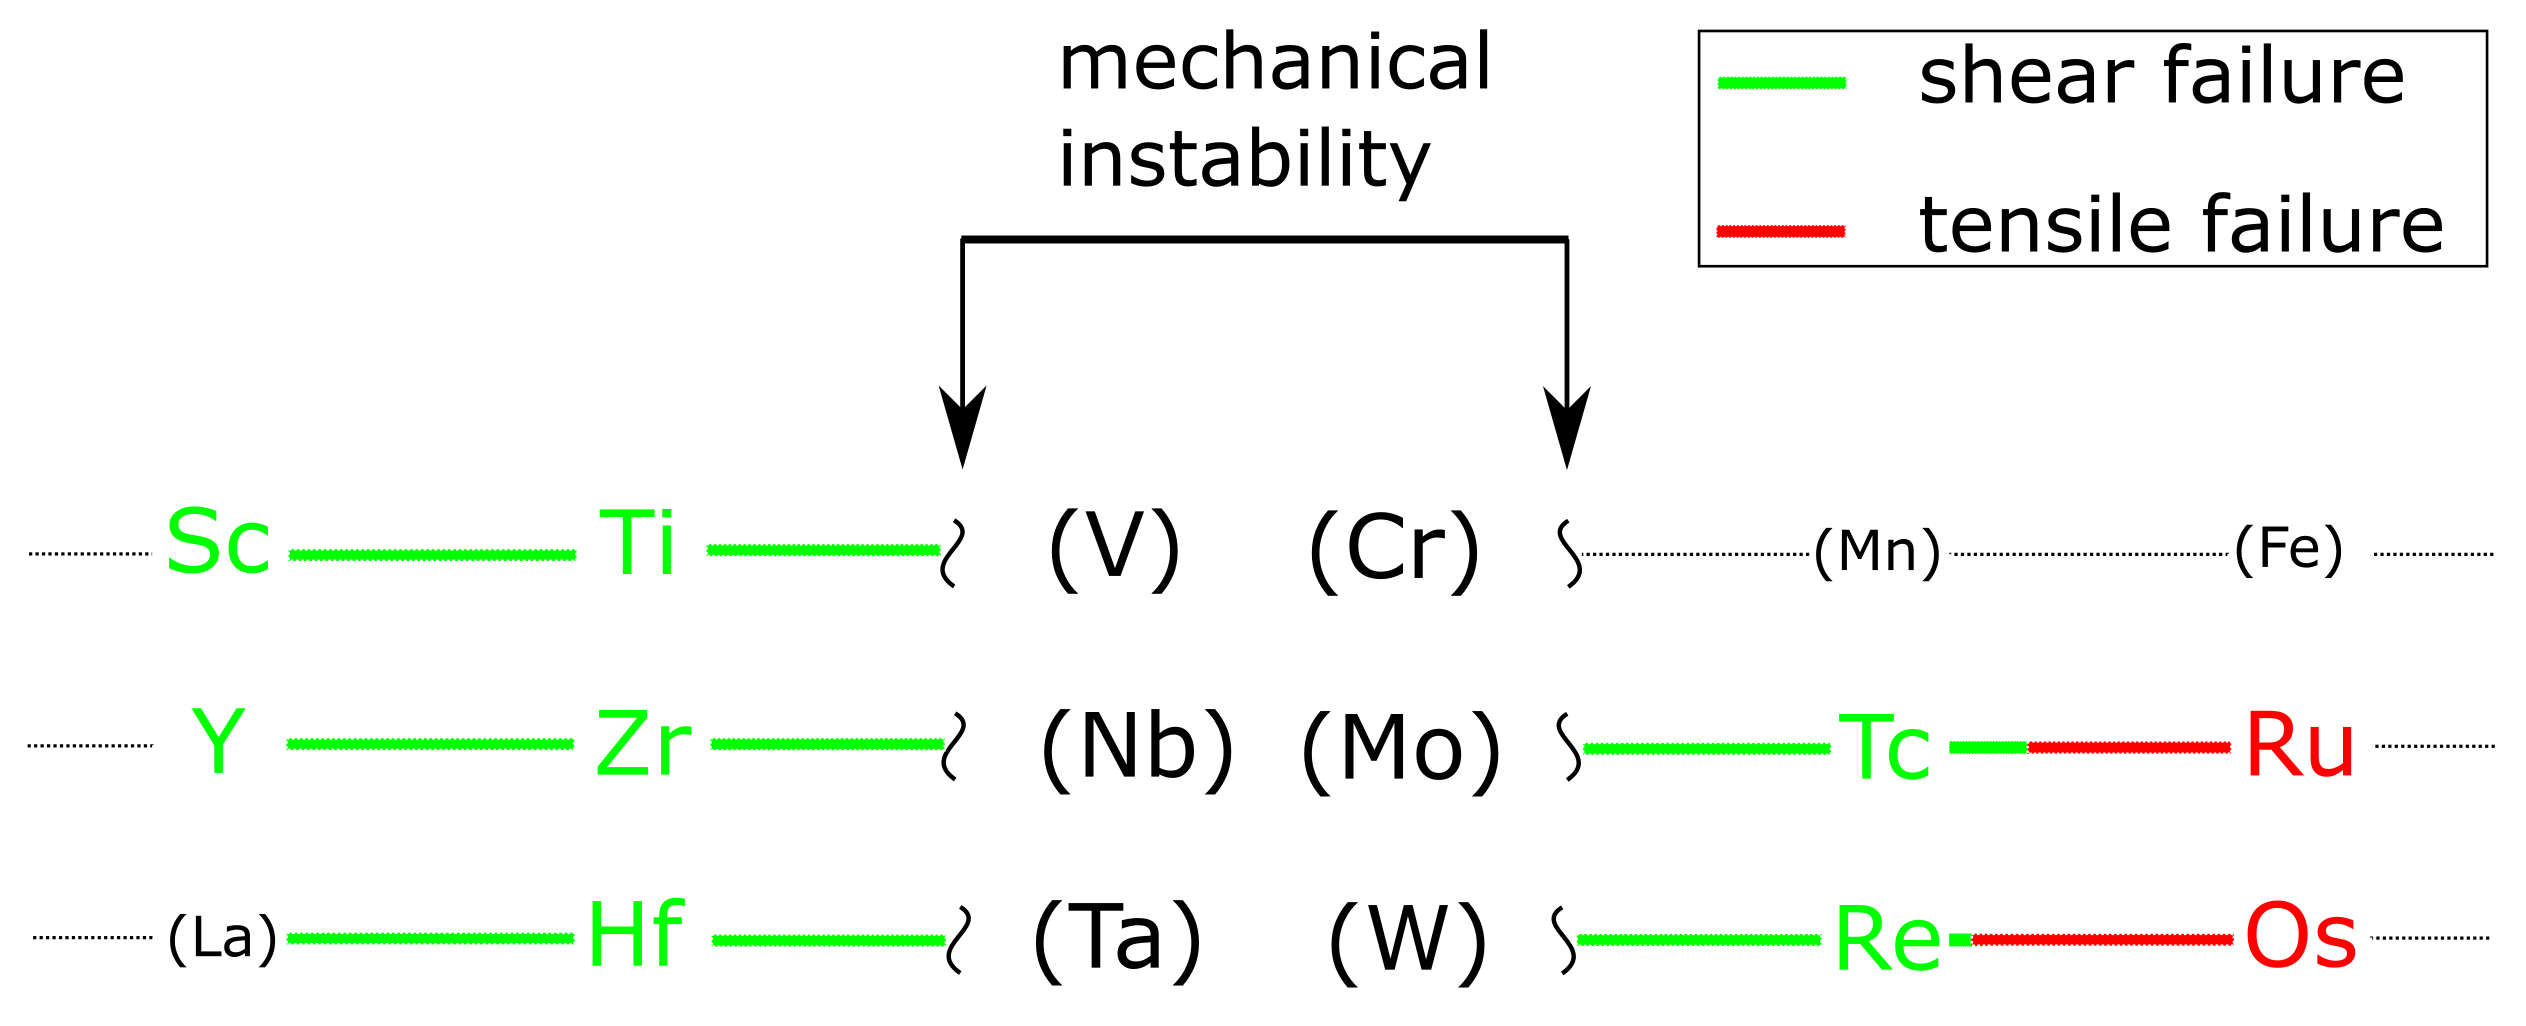
\includegraphics[width=0.50\textwidth]{drawing1.png}
\caption{Ideal failure mode-diagram vs. $d$-band filling in HCP metals and alloys}
\label{fig:sgentwinpic1}
\end{figure}

Moving to the right of the periodic table, we note that the group VII HCP-metals Re and Tc fail in shear and are hence intrinsically ductile. The metal Re is of particular interesting, as it exhibits the highest shear modulus among all HCP metals that fail in shear, suggesting the interesting combination of high strength and ductility. Moving further to the right, we note the metals Ru and Os in group VIII, exhibiting the highest shear moduli among all HCP-metals and almost all other elements in the periodic table. These fail in tension when loaded along $c$, largely due to their very high shear moduli. Small perturbations in $d$-band filling towards lower values do not change the ideal deformation behavior and the intrinsically brittle failure mode is maintained all the way up to $d$-band fillings close to group VII.

The formalism based on SOEC's and TOEC's developed in this work can be used to understand the features of the elastic response underlying shear versus tensile failure. Consider first HCP materials with high shear moduli, $C_{44}$, such as Ru and Os. These materials are not likely to fail in shear, since the eigenvalue associated with shear failure (Eq. \ref{eqn:Wallace3}) is rather large and may not reach zero before the eigenvalue in Eq. \ref{eqn:Wallace4}. Hence, this observation explains from an ideal strength point of view why the HCP metals that are most stiff in shear, and thus expected to have high strangth, tend to be brittle under $c$-axis loading. Strong materials with a high shear modulus $C_{44}$ will only fail in shear and be accordingly intrinsically ductile according to Eq. \ref{eqn:Wallace3} if $\sigma_{33}$ is relatively large in magnitude, requiring that $C_{33}$ is large. Further, the modulus $C_{333}$ is negative for most materials, implying softening of $C_{33}$ as the materials is strained along $c$ by $\xi$. A small magnitude of $C_{333}$ is also favorable for shear failure as it causes the magnitude of the stress $\sigma_{33}$ decrease less rapidly as a function of $\xi$.

Metals and alloys near half $d$-band filling, such as Re and Tc, are intrinsically ductile and fail in shear but are on the border of $d$-band filling regions where tensile failure occurs. Their shear failure is caused by an interplay of the SOEC's and TOEC's. First, the shear moduli $C_{44}$ of Re and Tc are large but smaller than those for Os and Ru. The same is true for the moduli $C_{33}$, but the ratio $C_{33}/C_{44}$ for group VII metals is larger than for group VIII: for Os  $C_{33}/C_{44} \approx 3.2$ whereas for Re $C_{33}/C_{44} \approx 4.5$. Second, for group VII metals, the magnitude of $C_{333}$ is smaller than for group VIII, which also promotes shear failure over tensile failure. Third, the TOEC $C_{344}$, which is a negative quantity for most materials, is relatively large in magnitude for group VII metals, relative to those in group VIII. According to Eq. \ref{eqn:Cprime} (e), this implies that the shear modulus $C_{44}$ decreases relatively rapidly with strain $\xi$, which according to Eq. \ref{eqn:Wallace3}, favors a shear instability over a tensile instability. 

Finally, the high ductility HCP metals in group IV exhibit values of $C_{33}/C_{44}$ between approximately 4 and 6 which is higher than for groups VII and VIII. The relatively low values for $C_{44}$ causes the eigenvalue in Eq. \ref{eqn:Wallace3} to attain negative values before the eigenvalue in Eq. \ref{eqn:Wallace4}, and consequently to fail in shear.

\section{Summary and Conclusions}
In this work, the ideal deformation behavior and elastic stabilities of 12 HCP metals under uniaxial stress along the $c$-axis are studied: Be, Mg, Sc, Y, Ti, Zr, Hf, Tc, Re, Ru, Os and Zn. It is found that out of these, 5 fail in tension along $c$ (Be, Mg, Ru, Os and Zn) whereas the 7 others (Sc, Y, Ti, Zr, Hf, Tc and Re) fail in shear. This leads to a natural division of the HCP metals into 2 classes: those that are intrinsically ductile (i.e., fail in shear) or intrinsically brittle (i.e., fail in tension) under tensile loads along $c$. Using a formalism based on the expansion of the elastic energy to third order in strain, it is further shown that the critical strain and the deformation mode can be predicted from the relative magnitudes of these  of the second and third order elastic constants.  It is found that HCP metals exhibiting high moduli $C_{44}$ tend to fail in tension rather than shear and hence, are intrinsically brittle. This occurs for transition metals and alloys in group VIII (Os, Ru). The HCP metals in groups III and IV are found to be intrinsically ductile under $c$-axis loading, primarily due to their low shear moduli $C_{44}$, which promotes shear failure. The group VII HCP metals (Re, Tc) are an interesting case that combine a high shear modulus with intrinsically ductile behavior. The physical reason for this behavior is the specific combination of SOEC's and TOEC's that this class of materials exhibits: a high $C_{33}$, but a relatively small magnitude of $C_{333}$ and a large magnitude of $C_{344}$. Finally, the trends of the ideal deformation behavior with $d$-band filling are revealed, resulting in approximate $d$-electron counts per atom for which an alloy is expected to fail in a ductile or brittle mode.

\appendix
\section{}
The imposed strain along $c$ ($\xi$) and the resulting strain in the basal plane ($\eta$) required to ensure zero normal stress within the basal plane are related by the Poisson's ratio for small strains. For large values of $\xi$, however, the TOEC's have to be invoked to calculate $\eta$.

Consider the mapping between the reference and current configuration of a continuum solid. In the reference configuration, a particle occupies a point $\bm{p}$ with spatial coordinates $\bm{X} = X_{1}\bm{e}_{1} +  X_{2}\bm{e}_{2} + X_{3}\bm{e}_{3}$, where ${e}_{1}, {e}_{2}, {e}_{3}$ is a Cartesian reference triad and $X_{1}, X_{2}, X_{3}$ are the reference coordinates. Upon deformation of the body, the point originally at $\bm{X}$ is translated by the displacement vector $\bm{u} \left(X_{1}, X_{2}, X_{3} \right)$ to its final coordinates $\bm{x} \left(X_{1}, X_{2}, X_{3} \right)$, see Eq. \ref{eqn:displ1} .
\begin{equation}
\label{eqn:displ1} 
\bm{x} \left(X_{1}, X_{2}, X_{3} \right) = \bm{u} \left(X_{1}, X_{2}, X_{3} \right) + \bm{X} \left(X_{1}, X_{2}, X_{3} \right)
\end{equation}

Based on this description, a deformation gradient is formulated as in Eq. \ref{eqn:defgrad1}. The Green-Lagrange strain tensor $\bm{\eta}$ then follows from $\bm{F}$ as shown in Eq. \ref{eqn:GL1}, where $\bm{I}$ denotes the identity matrix.
\begin{equation}
\label{eqn:defgrad1} 
\bm{F} = \frac{\partial x_{i}}{ \partial X_{j}}
\end{equation}

\begin{equation}
\label{eqn:GL1} 
\bm{\eta} = \frac{1}{2} \left(\bm{F}^{T} \bm{F} - \bm{I} \right)
\end{equation}

With the notation now established, the strain energy density can be expanded in terms of the SOEC's, TOEC's and the Green-Lagrange strain  as in Eq. \ref{eqn:expansion1}, where $\rho_{0}$ represents the mass density in the undeformed state and the terms $\eta_{i}$ represent the components of the tensor defined in Eq. \ref{eqn:GL1}. The symmetry of the SOEC's and TOEC's will be applied in the expansions, which simplifies the resulting expressions considerably.

\begin{equation}
\label{eqn:expansion1} 
\rho_{0} E \left(\bm{\eta}\right) = \frac{1}{2!} \sum_{i,j=1}^{6} C_{ij} \eta_{i} \eta_{j} + \frac{1}{3!} \sum_{i,j,k=1}^{6} C_{ijk} \eta_{i} \eta_{j} \eta_{k} + \ldots
\end{equation}

Consider an imposed strain $\xi$ along the $c$-axis of an HCP-metal, initially keeping all other dimensions fixed to the zero strain-state. Consider first the expansion of Eq. \ref{eqn:expansion1}, retaining only terms up to and including the SOEC's (hence, ignoring the TOEC's for now). This gives the energy-expression in Eq. \ref{eqn:expansion3}, in which the symmetry of the SOEC's has been applied. To obtain the equilibrium strain in the basal plane due to the application of $\xi$, we perform strain energy-minimization and set $\bar{\eta} = \eta = \eta_{1} = \eta_{2}$, $\eta_{3} = \xi$ and $\eta_{4} = \eta_{5} = \eta_{6} = 0$ in Eq. \ref{eqn:expansion3} and solve $\frac{\partial \left(\rho_{0} E\right)}{\partial \eta}|_{\xi} = 0$. We find the equilibrium strain $\eta = \bar{\eta}$, given in Eq. \ref{eqn:eqstr1}, where the minus-sign signifies the Poisson-contraction in the basal plane.

\begin{multline}
\label{eqn:expansion3} 
\rho_{0} E \left(\bm{\eta}\right) = C_{11}\frac{\eta_{1}^2}{2} + C_{11}\frac{\eta_{2}^2}{2} +  C_{33}\frac{\xi^2}{2} + C_{44}\frac{\eta_{4}^2}{2} + C_{44}\frac{\eta_{5}^2}{2} + \\  \frac{1}{2} \left(C_{11}-C_{12}\right)\frac{\eta_{6}^2}{2} + C_{12}\eta_{1}\eta_{2} + C_{13}\eta_{1}\xi + C_{13}\eta_{2}\xi
\end{multline}

\begin{equation}
\label{eqn:eqstr1} 
\eta = \bar{\eta} = -\frac{\xi C_{13}}{C_{11} + C_{12}}
\end{equation}

For large strains, the expansion in Eq. \ref{eqn:expansion3} is not sufficient and instead, TOEC's have to be included as well. The expansion of the strain energy up to the third order in strain is given in Eq. \ref{eqn:expansion2}, in which the terms $P$ are given in Eq. \ref{eqn:expansion2detailed}. Note that in Eq. \ref{eqn:expansion2}, the symmetry of the SOEC's and TOEC's has been incorporated to simplify the resulting expression. 

\begin{multline}
\label{eqn:expansion2} 
\rho_{0} E \left(\bm{\eta}\right) = C_{11} P_{1} +  C_{12} P_{2} + C_{13} P_{3} + C_{33} P_{4} + \\ C_{44} P_{5} + C_{111} P_{6} + C_{222} P_{7} + C_{333} P_{8} + \\ C_{133} P_{9} +  C_{113} P_{10} + C_{112} P_{11} + C_{123} P_{12} + \\ C_{144} P_{13} + C_{155} P_{14} + C_{344} P_{15}
\end{multline}


\begin{subequations}
\label{eqn:expansion2detailed} 
\begin{align}
        P_{1} &=\frac{\eta_{1}^2}{2}  + \frac{\eta_{2}^2}{2} + \frac{\eta_{6}^2}{4} ,\\
       P_{2} &=-\frac{\eta_{6}^2}{4} + \eta_{1}\eta_{2} ,\\
				P_{3} &=\eta_{1}\eta_{3} + \eta_{2}\eta_{3} , \\
				P_{4} &=\frac{\eta_{3}^2}{4} , \\
				P_{5} &=\frac{\eta_{4}^2}{2} + \frac{\eta_{5}^2}{2} , \\
				P_{6} &=\frac{\eta_{1}^3}{6} + \frac{\eta_{1}\eta_{2}^2}{2} - \frac{\eta_{1}\eta_{6}^2}{4} + \frac{\eta_{2}\eta_{6}^2}{4} , \\
				P_{7} &=\frac{\eta_{2}^3}{6} - \frac{\eta_{1}\eta_{2}^2}{2} - \frac{\eta_{2}\eta_{6}^2}{8} + 3\frac{\eta_{1}\eta_{6}^2}{8} , \\
				P_{8} &=\frac{\eta_{3}^3}{6} , \\
				P_{9} &=\frac{\eta_{1}\eta_{3}^2}{2} + \frac{\eta_{2}\eta_{3}^2}{2} , \\
				P_{10} &=\frac{\eta_{3}\eta_{1}^2}{2} + \frac{\eta_{3}\eta_{2}^2}{2} + \frac{\eta_{3}\eta_{6}^2}{4} , \\
				P_{11} &=\frac{\eta_{1}^2\eta_{2}}{2} +  \frac{\eta_{1}\eta_{2}^2}{2} - \frac{\eta_{6}^2\eta_{1}}{8} - \frac{\eta_{6}^2\eta_{2}}{8} , \\
				P_{12} &=\eta_{1}\eta_{2}\eta_{3} - \frac{\eta_{3}\eta_{6}^2}{4} , \\
				P_{13} &=\frac{\eta_{1}\eta_{4}^2}{2} + \frac{\eta_{2}\eta_{5}^2}{2} - \frac{\eta_{4}\eta_{5}\eta_{6}}{2} , \\
				P_{14} &=\frac{\eta_{2}\eta_{4}^2}{2} + \frac{\eta_{1}\eta_{5}^2}{2} + \frac{\eta_{4}\eta_{5}\eta_{6}}{2} , \\
				P_{15} &=\frac{\eta_{3}\eta_{4}^2}{2} + \frac{\eta_{3}\eta_{5}^2}{2} 
\end{align}
\end{subequations}

Given an applied $\xi$, we can again find an analytical expression for the Poisson contraction $\eta = \bar{\eta}$ in terms of $\xi$ and the SOEC's and TOEC's. The resulting equation that has to be solved is shown in Eq. \ref{eqn:minexpression1}. Solving Eq. \ref{eqn:minexpression1} in terms of $\eta = \bar{\eta} = \eta_{1} = \eta_{2}$ gives the equilibrium strain in the basal plane.

\section{}
A simple expression for the relations between strains and stresses can be derived for an HCP-structured material that is loaded in tension along the $c$-axis, while allowing for contraction in the basal plane. For this situation, with an applied (Lagrangian) strain $\eta_{3}$ along $c$, we have $\eta_{1}=\eta_{2}=\bar{\eta}$ and $\eta_{3}=\xi$ . Eq. \ref{eqn:stressexpansion1} expresses the Lagrangian stress tensor in terms of the strain energy and Lagrangian strain tensor \cite{lopuszynski2007ab}. From Eq. \ref{eqn:stressexpansion1}, the Lagrangrian stress $t_{33}$ can be found under the combined strain state currently under investigation, see Eq. \ref{eqn:t33eq1}. Further, from Eq. \ref{eqn:stressconversion1}, we have that $\bm{\sigma} = \frac{1}{\text{det} \left(\bm{F}\right)} \bm{F} \bm{t} \bm{F}^{T}$ which governs the relation between Lagrangian and true stress. This expression can be expanded, with the result given in Eq. \ref{eqn:t33eq2}, where $t_{33}$ is given in Eq. \ref{eqn:t33eq1}. 


%We first derive an expression for the true stress component $\sigma_{33}$. Eq. \ref{eqn:stressexpansion1} expresses the Lagrangian stress tensor in terms of the strain energy and Lagrangian strain tensor \cite{lopuszynski2007ab}. Eq. \ref{eqn:stressexpansion1} is employed to calculate the Lagrangian stress $t_{33}$, under a combined loading condition of $\eta_{1}=\eta_{2}=\bar{\eta}$ and $\eta_{3}=\xi$ simultaneously. The result is shown in Eq. \ref{eqn:t33eq1}. From Eq. \ref{eqn:stressconversion1}, we have that $\bm{\sigma} = \frac{1}{\text{det} \left(\bm{F}\right)} \bm{F} \bm{t} \bm{F}^{T}$. This expression can be expanded, with the result given in Eq. \ref{eqn:t33eq2}, where $t_{33}$ is given in Eq. \ref{eqn:t33eq1}. 

\begin{equation}
\label{eqn:stressexpansion1} 
t_{ij} = \rho_{0} \frac{\partial E}{\eta_{ij}}
\end{equation}

\begin{multline}
\label{eqn:t33eq1} 
t_{33} \Bigr|_{\eta_4=\eta_5=\eta_6=0}  = \eta_{1}^{2} \left(C_{113} + C_{123} \right) + \eta_{1} \left(2C_{13} + 2C_{133}\eta_{3} \right) + \\ \frac{1}{2} C_{333} \eta_{3}^{2} + C_{33} \eta_{3}
\end{multline}

\begin{equation}
\label{eqn:stressconversion1} 
t_{ij} = \text{det} \left(\bm{F}\right) \bm{F}^{-1} \bm{\sigma} \left(\bm{F}^{T}\right)^{-1}
\end{equation}

\begin{equation}
\label{eqn:t33eq2} 
\sigma_{33}  = \frac{\sqrt{2 \xi + 1}}{\sqrt{2 \bar{\eta} + 1}}t_{33}
\end{equation}


\bibliography{refs.bib}

\end{document} %EOPAPER

